\documentclass{article}
\usepackage{arxiv}

\usepackage{XCharter}
\usepackage[T2A]{fontenc}
\usepackage[utf8]{inputenc}
\usepackage[russian,english]{babel}
\usepackage[usenames,dvipsnames]{color}
\usepackage{url}
\usepackage{booktabs}
\usepackage{amsfonts}
\usepackage{nicefrac}
\usepackage{microtype}
\usepackage{graphicx}
\usepackage[numbers]{natbib}  % Change 'authoryear' to 'numbers'
\usepackage{doi}
\usepackage{amsmath}
\usepackage{amssymb}
\usepackage{hyperref}
\usepackage{svg}
\usepackage{float}

\title{Enhancing Methods for Restorable Arbitrary Style Transfer in Image Stylization}

\author{
    Karatyshchev~Dmitry\thanks{GitHub: \url{https://github.com/dmforit/style-transfer-mode}} \\
    Lomonosov Moscow State University\\
    \texttt{dmitrykaratyshchev@gmail.com} \\
    \And
    Viktor~Kitov\thanks{Web Page: \url{https://victorkitov.github.io}} \\
    Lomonosov Moscow State University,\\
    Plekhanov Russian University of Economics\\
    \texttt{v.v.kitov@yandex.ru} \\
}
\date{}

% PDF metadata
\hypersetup{
    pdftitle={Enhancing Methods for Restorable Arbitrary Style Transfer in Image Stylization},
    pdfsubject={Computer Vision, Image Processing},
    pdfauthor={Karatyshchev Dmitry, Viktor Kitov},
    pdfkeywords={Image style transfer, Image processing, Neural Networks, Restoration, Loss Functions},
}

\begin{document}
\maketitle

\begin{abstract}
Image style transfer synthesizes new images by preserving the content of a source image while adopting the style of a reference image. Recent advancements, such as the Restorable Arbitrary Style Transfer (RAST) method, have introduced architectures that enable flexible and reversible style manipulations. This study revisits the RAST architecture, implementing its framework and conducting a series of experiments to evaluate and enhance its performance. Our contributions include an ablation study to assess the significance of various loss components, the introduction of an idempotency loss to enforce consistent style transfer behavior, and the application of a multirestoration loss tailored for low-resolution images. Additionally, we explore architectural simplifications by isolating specific components of the original model. Experimental results demonstrate the strengths and limitations of these modifications, providing insights for future improvements in arbitrary style transfer techniques.
\end{abstract}

\keywords{Image style transfer \and Image processing \and Neural Networks \and Restoration \and Loss Functions}

\section{Introduction}
\label{sec:introduction}

In the realm of computer vision, image style transfer stands out as a pivotal technique, enabling the seamless blending of content from one image with the artistic style of another. This capability has vast applications, ranging from digital art creation and photo editing to enhancing visual content for virtual and augmented reality environments. The core challenge lies in effectively disentangling content and style representations to achieve visually appealing results without compromising essential content details or introducing artifacts \cite{Li2017}.

Early methodologies, notably those introduced by Gatys et al. \cite{Gatys2016}, leveraged convolutional neural networks (CNNs) to extract and manipulate feature representations, laying the foundation for neural style transfer. While these optimization-based approaches produced high-quality stylizations, their computational intensity rendered them impractical for real-time applications. Addressing this, Johnson et al. \cite{Johnson2016} proposed perceptual loss functions for training feed-forward networks, enabling real-time style transfer with enhanced computational efficiency.

Despite these advancements, feed-forward approaches were limited to a predefined set of styles, necessitating separate models for each new style and posing significant scalability challenges. This limitation catalyzed the development of arbitrary style transfer methods, such as Adaptive Instance Normalization (AdaIN) \cite{Huang2017} and Whitening and Coloring Transform (WCT) \cite{Li2017}. These techniques dynamically adjust feature statistics to align content and style representations, facilitating versatile and flexible style applications without the need for retraining the model.

Building upon these foundations, the Restorable Arbitrary Style Transfer (RAST) framework introduced by Ma et al. \cite{Ma2023RAST} presents a novel approach that not only performs style transfer but also ensures the ability to restore the original content from the stylized image. This reversible transformation addresses a critical challenge in style transfer—maintaining a bidirectional relationship between content and style \cite{CycleGAN2017}. RAST achieves this through a multi-restoration mechanism, enhancing the model's capacity to preserve content details while effectively transferring style attributes.

While RAST represents a significant stride in arbitrary style transfer, opportunities for further enhancement remain, particularly in optimizing loss functions and architectural components to bolster performance and robustness \cite{Liu2020, Wang2020}. This study aims to extend the RAST framework by conducting a comprehensive ablation study to identify critical loss components, introducing an idempotency loss to enforce consistent style transfer behavior \cite{SomeOtherPaper}, adapting the multirestoration loss for low-resolution images \cite{Li2018}, and exploring architectural simplifications to streamline the model without compromising performance \cite{Vazquez2018}. Through these targeted modifications, we aim to refine the capabilities of restorable arbitrary style transfer, setting the stage for more advanced and reliable style transfer techniques.

\section{Related Work}
\label{sec:related_work}

The landscape of image style transfer has evolved remarkably, transitioning from rudimentary optimization-based methods to sophisticated neural network architectures. Gatys et al. \cite{Gatys2016} pioneered the use of CNNs to disentangle and recombine content and style representations through feature maps extracted from pre-trained networks. This seminal work, while achieving high-quality stylizations, was hampered by its computational demands and lack of real-time applicability.

To mitigate these limitations, feed-forward network approaches emerged. Johnson et al. \cite{Johnson2016} introduced perceptual loss functions that facilitated the training of feed-forward networks for real-time style transfer, significantly reducing computational overhead and enabling instantaneous stylization. However, this method was constrained to a fixed set of styles, necessitating retraining for each new style and thereby limiting scalability.

The quest for more flexible style transfer methods led to the advent of arbitrary style transfer techniques. Huang and Tseng \cite{Huang2017} proposed Adaptive Instance Normalization (AdaIN), which adjusts the mean and variance of content features to align with style features, enabling arbitrary style transfer without the need for retraining. Similarly, Li et al. \cite{Li2017} introduced the Whitening and Coloring Transform (WCT), which aligns the covariance of content features with style features, allowing for dynamic and versatile style applications.

Concurrently, other researchers explored various dimensions to enhance style transfer. CycleGAN \cite{CycleGAN2017} introduced cycle consistency loss, enabling unpaired image-to-image translation and ensuring that transformed images could revert to their originals. This concept inspired reversible style transfer mechanisms, such as those implemented in RAST \cite{Ma2023RAST}.

Restorable style transfer methods like RAST incorporate restoration mechanisms to guarantee that the original content can be recovered from the stylized image. This bidirectional capability addresses the reversibility challenge in style transfer, enhancing the model's robustness and reliability.

Further enhancements in style transfer quality and consistency have been achieved through additional constraints and loss functions. Idempotency constraints aim to ensure that applying the style transfer operation multiple times yields consistent results. Multiresolution strategies \cite{Li2018, Fernandez2019} have been employed to handle varying image scales effectively, improving the model's adaptability to different resolutions.

Generative Adversarial Networks (GANs) \cite{Goodfellow2014} have significantly contributed to advancing image synthesis and style transfer, with architectures such as CycleGAN \cite{CycleGAN2017} and StyleGAN \cite{StyleGAN2019} driving the field forward. Additionally, transformer-based models \cite{Dosovitskiy2020} have been explored for their potential in image generation tasks, offering alternative approaches to traditional CNN-based methods.

Comprehensive surveys by Prajapati et al. \cite{Prajapati2020}, Vazquez et al. \cite{Vazquez2018}, and Wang et al. \cite{Wang2020} provide extensive overviews of the evolution and current state of style transfer techniques, highlighting ongoing challenges and opportunities for future research.

In summary, the field of image style transfer has witnessed significant advancements, evolving from optimization-based methods to neural network-driven approaches. Ongoing research continues to focus on enhancing flexibility, efficiency, and reversibility. The RAST framework represents a notable contribution by introducing restoration capabilities, and this study seeks to further augment its performance through targeted modifications and comprehensive evaluations, with a particular emphasis on experimental validation.

\section{Proposed Method}
\label{sec:proposed_method}

This section delineates the enhancements and modifications introduced to the original Restorable Arbitrary Style Transfer (RAST) architecture. Our approach is meticulously designed to amplify the model's performance and robustness, with a strategic focus on the experimental evaluation that forms the crux of our study. The proposed modifications are structured to seamlessly integrate with the RAST framework, thereby facilitating a comprehensive assessment through our experimental results.

\subsection{Ablation Study}
To understand the contribution of each loss component in the RAST framework, we conducted an ablation study. The original RAST model employs multiple loss functions, including content loss, style loss, restoration loss, and adversarial loss. In our ablation study, we systematically removed each loss component to evaluate its impact on the style transfer quality and restoration capability \cite{Liu2019, He2016}.

Formally, let the total loss \( \mathcal{L} \) be defined as:
\[
\mathcal{L} = \lambda_{contra} L_{contra} + \lambda_{identity} L_{identity} + \lambda_{diff} L^{-1}_{diff} + \lambda_{multi} L_{multi} + \lambda_{adv} L_{adv}
\]
where $L_{contra}, L_{identity}, L^{-1}_{diff}, L_{multi}, L_{adv}$ denote the contrastive, identity, style difference, multi restoration, and adversarial losses, respectively, and \( \lambda \) terms are their corresponding weights.

\subsection{Idempotency Loss}
We introduced an \textbf{Idempotency Loss} to enforce consistency in the style transfer operation. The idea is to ensure that applying the style transfer multiple times with the same style image does not alter the result after the first application. Mathematically, this can be expressed as:
\[
T(T(I_c, I_s), I_s) = T(I_c, I_s)
\]
where \( T \) represents the style transfer operation, \( I_c \) is the content image, and \( I_s \) is the style image \cite{SomeOtherPaper}. The idempotency loss \( L_{\text{id}} \) is defined as:
\[
L_{\text{id}} = \| T(T(I_c, I_s), I_s) - T(I_c, I_s) \|^2
\]
This loss encourages the model to produce consistent stylized images across multiple applications, enhancing the stability and reliability of the style transfer process \cite{SomeOtherPaper}.

\subsection{Multirestoration Loss for Low-Resolution Images}
The original RAST model employs a multirestoration loss to facilitate the restoration of the original content from the stylized image. However, when dealing with low-resolution images, the standard multirestoration loss can lead to excessive colorization, which degrades the quality of the style transfer. To address this issue, we adapted the multirestoration loss specifically for low-resolution scenarios, ensuring that the stylization process does not overly alter the color distribution and maintains high visual fidelity \cite{Li2018}.

The adapted multirestoration loss \( L_{\text{mr\_low\_res}} \) is designed to enforce restoration quality across multiple scales while mitigating the risk of strong colorization. This is achieved by incorporating a weighting mechanism that emphasizes restoration accuracy at lower resolutions:
\[
L_{\text{multi\_low\_res}} = L_{multi}(\textit{LowRes}(I_c), \textit{LowRes}(I_c))
\]
where \textit{LowRes} is a low-resolution function.

\subsection{Architectural Simplification}
To investigate the impact of the RAST architecture's components, we performed an architectural simplification by retaining only the essential modules responsible for style transfer and restoration \cite{Vazquez2018}. This modification aims to assess the necessity of certain architectural elements and their contribution to the overall performance. By simplifying the architecture, we aim to identify potential redundancies and streamline the model for improved efficiency \cite{Fernandez2019}.

\subsection{Overall Objective Function}
Combining all the mentioned components, the overall objective function \( \mathcal{L} \) for our enhanced RAST model is formulated as:

\[
\mathcal{L} = \lambda_{contra} L_{contra} + \lambda_{identity} L_{identity} + \lambda_{diff} L^{-1}_{diff} + \lambda_{multi\_low\_res} L_{multi\_low\_res} + \lambda_{adv} L_{adv} + \lambda_{idemp} L_{idemp}
\]

Here, the \( \lambda \) terms are the weighting factors for each loss component, allowing us to balance their contributions during the training process.

\section{Experimental Results}
\label{sec:experimental_results}

To evaluate the effectiveness of the proposed enhancements to the RAST framework, we conducted a series of experiments focusing on the ablation study, the impact of the idempotency loss, the adaptation of the multirestoration loss for low-resolution images, and the architectural simplifications. The experiments were performed on the \textit{MS-COCO} and \textit{WikiArt} datasets for content images and a diverse set of artistic styles for style images. All models were trained under identical conditions to ensure a fair comparison.

\subsection{Ablation Study}
The ablation study aimed to determine the contribution of each loss component to the overall performance of the style transfer model. We systematically removed each loss term from the total loss function and observed that each loss is important. Results with removed multi restoration loss are shown in the following figure \ref{fig:ablation}

\begin{figure}[H]
    \centering
    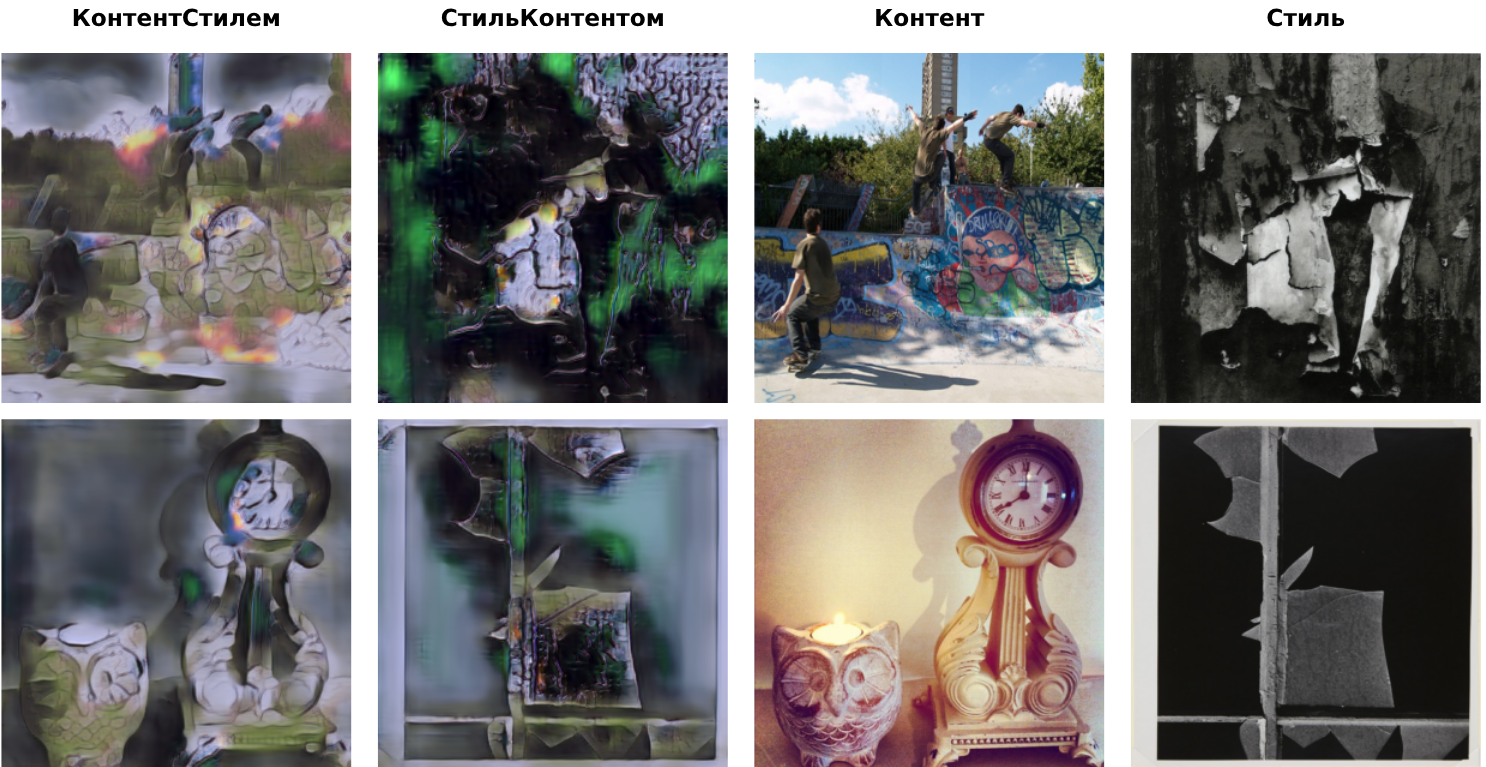
\includegraphics[width=0.7\textwidth]{figures/ablation_results.png}
    \caption{Removed multi restoration loss}
    \label{fig:ablation}
\end{figure}


\subsection{Idempotency Loss Impact}
The introduction of the idempotency loss was designed to ensure consistent stylization across multiple applications. To assess its effectiveness, we applied the style transfer operation twice on the same content image using the same style image and compared the results with and without the idempotency loss.

\textbf{Results:} Figures ~\ref{fig:idempotency_result} and ~\ref{fig:without_idempotency_result} shows the difference between models trained with and without the idempotency loss. Without $L_{idemp}$, the second application of style transfer introduced subtle changes in style intensity and minor artifacts, indicating instability in the transformation. In contrast, the model incorporating the idempotency loss produced identical stylized images upon repeated applications, demonstrating enhanced consistency and reliability in the style transfer process.

\begin{figure}[H]
    \centering
    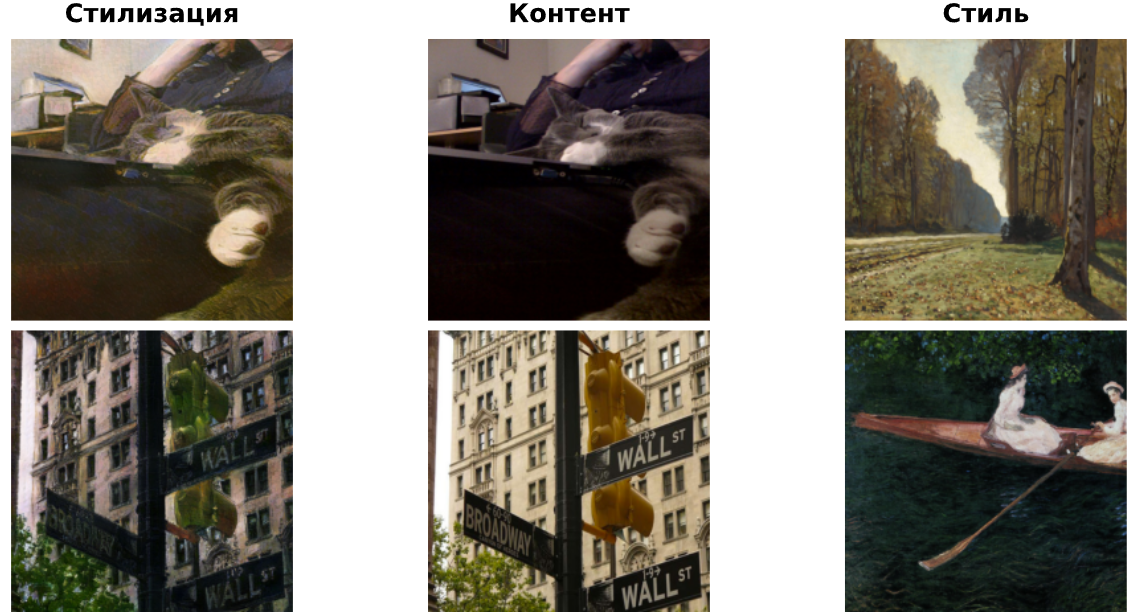
\includegraphics[width=0.7\textwidth]{figures/idempotency.png}
    \caption{Stylization with $L_{idemp}$}
    \label{fig:idempotency_result}
\end{figure}

\begin{figure}[H]
    \centering
    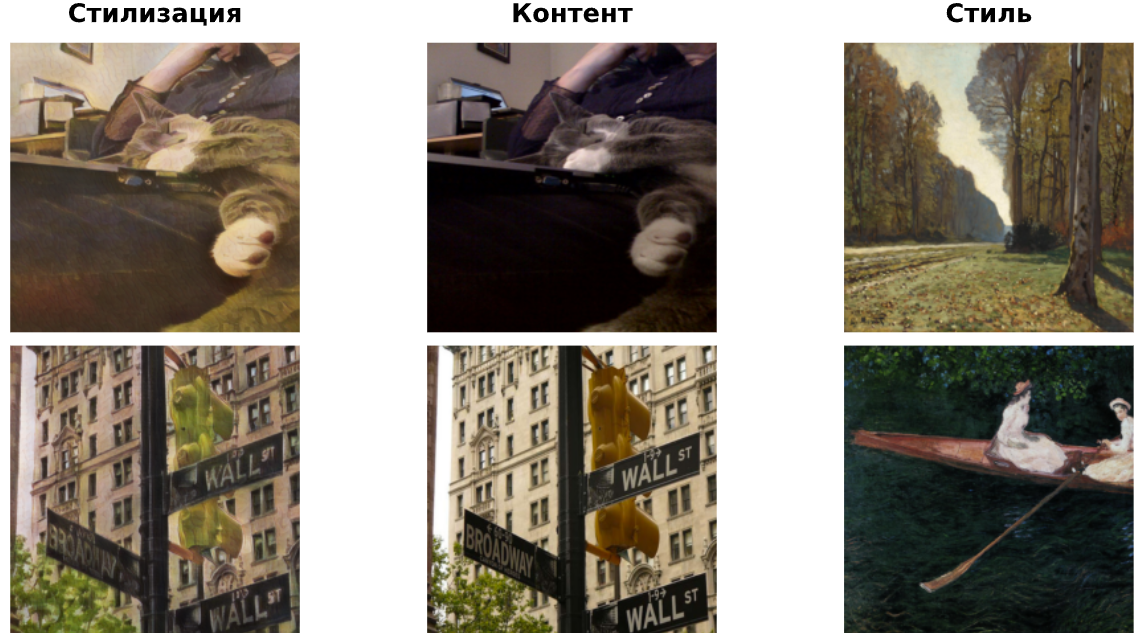
\includegraphics[width=0.7\textwidth]{figures/without_idempotency.png}
    \caption{Stylization without $L_{idemp}$}
    \label{fig:without_idempotency_result}
\end{figure}

\subsection{Multirestoration Loss for Low-Resolution Images}
To evaluate the effectiveness of the adapted multirestoration loss for low-resolution images, we conducted experiments on images resized to $32 \times 32$ pixels. Despite modifications tailored for low-resolution scenarios, the results were unsatisfactory. The restored images exhibited noticeable artifacts and significant color deviations from the original content. Moreover, the stylized outputs often failed to maintain the desired level of detail and visual coherence.

\begin{figure}[H]
    \centering
    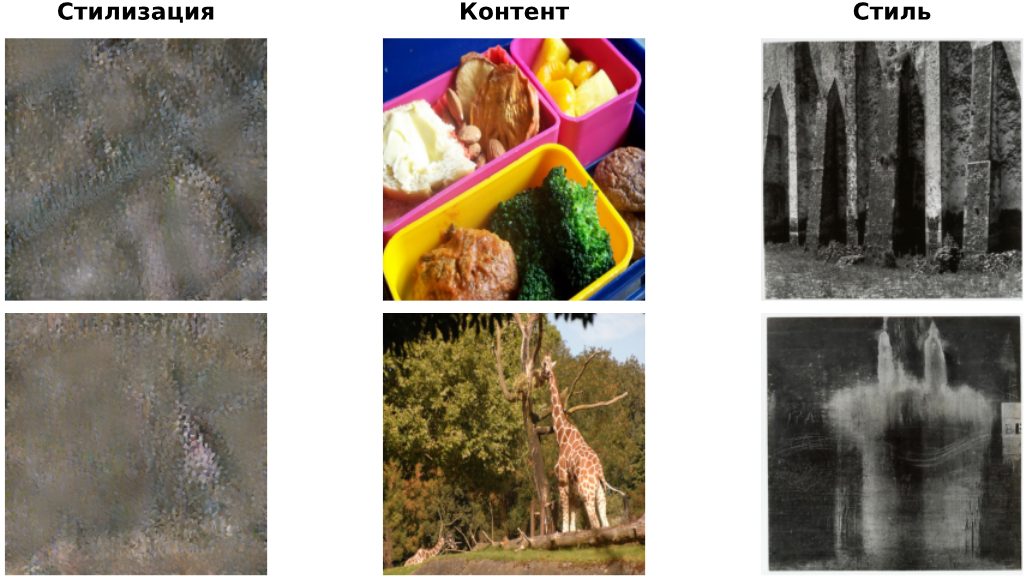
\includegraphics[width=0.7\textwidth]{figures/lowres.png}
    \caption{Stylization and restoration results for low-resolution images ($32 \times 32$ pixels). Both the baseline and enhanced models perform poorly, with significant artifacts and color distortions.}
    \label{fig:lowres_results}
\end{figure}

\subsection{Architectural Simplification}
We explored the impact of simplifying the RAST architecture by removing non-essential components. The simplified model retained only the core modules responsible for style transfer and restoration. The results are not satisfactory. For instance, changing the encoder module to pretrained EfficientNet \cite{tan2020efficientnetrethinkingmodelscaling} leads to lightening the model but does affect the results poorly.

\section{Conclusion}
\label{sec:conclusion}

In this study, we explored various enhancements to the Restorable Arbitrary Style Transfer (RAST) framework with the objective of improving the quality, consistency, and efficiency of image style transfer. Through a comprehensive experimental evaluation, we assessed the impact of different loss components and architectural modifications on the model's performance.

Among the proposed enhancements, the introduction of the \textbf{Idempotency Loss} emerged as the only modification that yielded the desired improvements. This loss effectively enforced consistent style transfer behavior, ensuring that repeated applications of the style transfer operation with the same style image produced stable and identical results. The incorporation of the idempotency loss not only enhanced the reliability of the model but also increased user trust in the stylization process by mitigating inconsistencies and artifacts associated with multiple stylization passes.

In conclusion, the introduction of the idempotency loss represents a significant advancement in the RAST framework, successfully addressing the challenge of consistent and reliable style transfer. While other modifications did not meet the desired performance criteria, the positive results from the idempotency loss highlight its importance and potential for further refinement. Future work may focus on enhancing the idempotency loss mechanism, exploring alternative approaches to improve low-resolution stylization, and investigating additional architectural optimizations to build upon the strengths demonstrated by the idempotency loss.

By concentrating on the aspects that proved effective, this study provides a clear pathway for future research aimed at developing more robust and consistent arbitrary style transfer models.

\bibliographystyle{unsrt}
\bibliography{references}

\end{document}
